\chapter{METODE PENELITIAN}
\label{chap:desainimplementasi}

% Ubah bagian-bagian berikut dengan isi dari desain dan implementasi

Tugas akhir ini merupakan peelitian pada bidang visi computer yang bertujuan untuk mengendalikan robot menggunakan metode \emph{classification} CNN. Secara umum metode yang digunakan adalah pertama pembuatan dataset, prediksi pose tangan, \emph{classification} menggunakan model CNN, dan terakhir navigasi control pada robot. Alur metodologi dapat dilihat pada

\begin{figure}[!h]
  \centering
	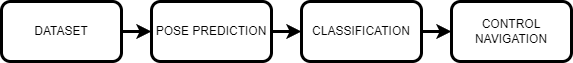
\includegraphics[width=1\linewidth]{gambar/metodologi.png}
	\caption{Blok diagram metodologi}
	\label{fig:metodologi}
\end{figure}

\section{Dataset}
\label{sec:deskripsisistem}

Tahapan pengambilan dataset dilakukan dengan mengambilan data-data berupa citra menggunakan kamera pada laptop. Kamera pada laptop dipakai untuk mendapatkan citra yang nantinya digunakan untuk mendeteksi suatu pose atau gestur tangan membutuhkan citra tangan untuk menemukan bagian tangan. Proses pengumpulan citra pose tangan yang digunakan sebagai navigasi robot  dimulai dengan menentukan jumlah kelas dataset. Kelas dataset berjumlah enam pose yang terdiri dari perintah maju, mundur, diam, belok kiri, belok kanan,dan tembak. Setiap pose membutuhkan dua tangan untuk memberikan perintah dengan telapak tangan dihadapkan ke arah kamera. Pose untuk perintah maju dilambangkan dengan kedua tangan mengepal. Pose mundur dilambangkan dengan meluruskan jari manis dan jari tengah seperti halnya pose angka dua pada SIBI pada kedua tangan dan telapak tangan.  Pose diam dilambangkan dengan membuka telapak tangan atau meluruskan semua jari pada kedua tangan.  Pose belok kiri dilambangkan dengan membuka telapak tangan pada tangan kiri dan mengepalkan tangan pada tangan kanan. Pose belok kanan merupakan kebalikan dari pose belok kiri yang dilambangkan dengan tangan kiri mengepal dan tangan kanan membuka telapak tangan. Pose tembak dilambangkan dengan meluruskan ibu jari dan jari manis sedangkan jari lain dikepalkan dengan jari manis diarahkan ke atas dan telapak tangan menghadap ke kamera.

\section{\emph{Pose prediction}}

Tangan yang terangkap kamera terdeteksi dengan bantuan framework Mediapipe. Framework Mediapipe ini memiliki 21 titik  \emph{keypoint} pada tangan. Proses mendeteksi tangan dimulai dengan cara mencari telapak tangan yang terdapat titik nol \emph{keypoint} yang disebut sebagai palm detection model. Setelah titik nol terdeteksi atau telapak tangan ditemukan kemudian mencari 20 titik lainnya pada tangan. Titik-titik \emph{keypoint} ini dicari menggunakan regresi. Setelah 21 titik \emph{keypoint} terdeteksi selanjutnya menyimpan koordinat x dan y dari yang relatif terhadap layar yang serta menghubungkan 21 titik tersebut sehingga membentuk \emph{hand landmark}. Rangka tiap tangan yang terdeteksi memiliki nilai-nilai koordinat pada tiap \emph{keypoint}, dari koordinat ini dicari nilai terkecil dan nilai terbesar.  Nilai-nilai ini nantinya digunakan untuk membuat bounding box pada setiap frame yang terdeteksi tangan didalamnya. Setiap frame memiliki dua bounding box dikarenakan harus terdapat dua tangan untuk bisa menavigasi robot. Bounding box ini digunakan untuk melakukan hand lokalisasi yang bertujuan untuk menormalisasi variasi posisi dari \emph{hand landmark} yang telah dibuat oleh Mediapipe. Hand lokalisasi ini nantinya membuang bagian citra diluar bounding box dan menyatukan kedua tangan setelahnya. Hasil dari hand lokalisasi nantinya disimpan pada suatu folder pada setiap class. Setelah seluruh data pada setiap class terpenuhi maka dilanjutkan tahapan selanjutnya yaitu \emph{training} dan \emph{classification}.

\section{\emph{Classification}}

\begin{figure}[!h]
  \centering
  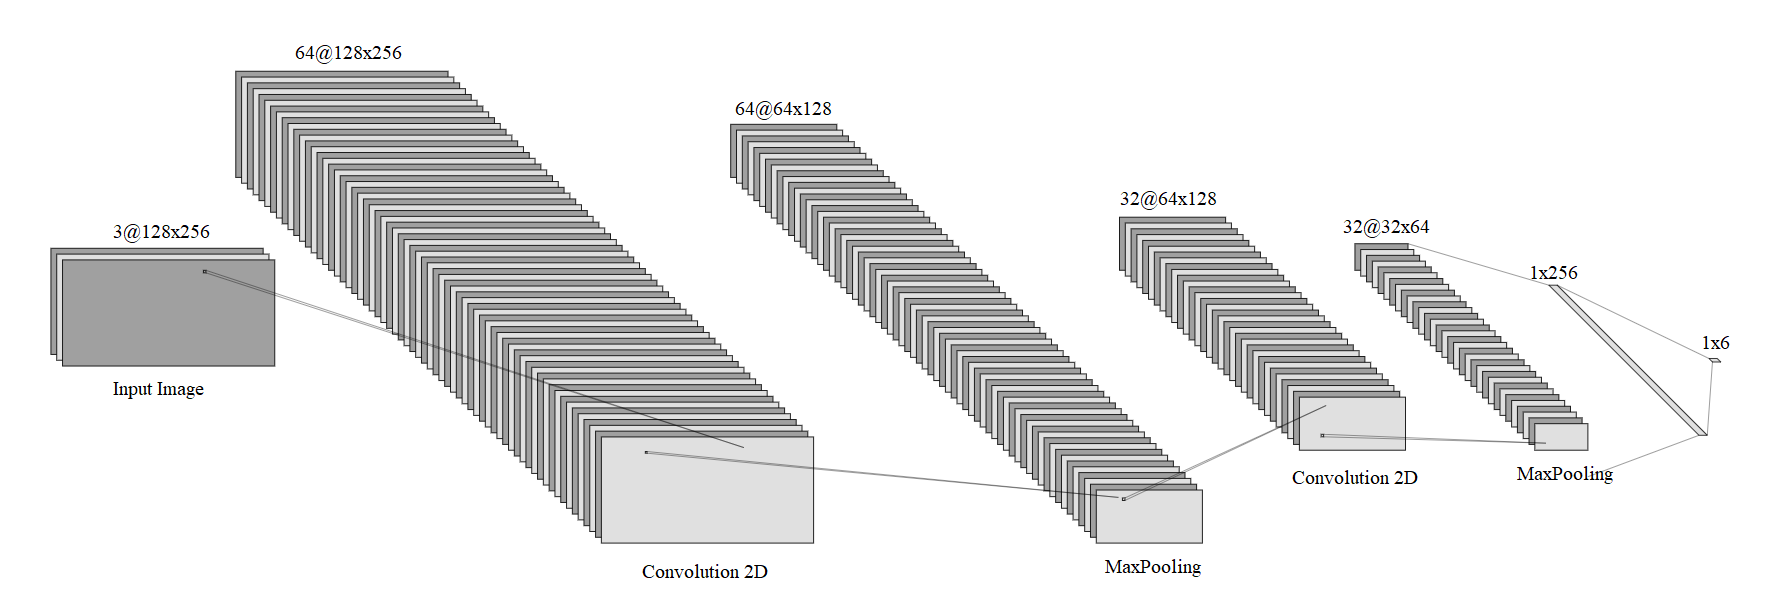
\includegraphics[width=1\linewidth]{../Gambar/LayerCnn.png}
  \caption{Layer CNN}
  \label{fig:layerCNn}
\end{figure}

Sebelum dilakukannya \emph{classification} dilakukan \emph{training} data terlebih dahulu. \emph{Training} data merupakan tahapan dari dataset yang telah dibuat yang kemudian dilatih untuk memperoleh suatu pola dari data tersebut. Pola tersebut digunakan untuk membantu mengenali objek dalam citra. Dalam proses \emph{training} dibutuhkan konfigurasi yang digunakan. Konfigurasi \emph{training} yang digunakan yaitu CNN dengan layer \emph{layer convolution}, \emph{layer max pooling},  dan flatten seperti yang ditampilkan pada Gambar \ref*{fig:layerCNn}. Adapun layer-layer tersebut membutuhkan konfigurasi seperti berikut :
\begin{enumerate}
  \item \emph{Convolution Layer}. \emph{Convolution layer} merupakan layer pertama dalam CNN yang melakukan proses konvolusi pada data citra untuk mengekstraksi fitur dari citra input sesuai dengan banyaknya filter yang digunakan \parencite{konvolusilayer}. 
  \item \emph{Pooling Layer}. \emph{Pooling layer} merupakan metode \emph{down-sumpling} yang bertujuan untuk mengurangi kompleksitas pada \emph{layer} selanjutnya. Pada penelitian ini akan dilakukan dengan metode max pooling yaitu mengambil nilai maksimal dari data citra dan bergerak dengan pergeseran \emph{layer} \parencite{poolilayer}.
  \item \emph{Fully-Connected Layer}. \emph{Fully-Connected layer} merupakan \emph{layer} yang digunakan untuk mengubah multidimensi data menjadi satu dimensi atau vektor. Layer ini digunakan setelah layer konvolusi dan pooling telah dilaksanakan. Cara kerja dari \emph{Fully-Connected layer} adalah memberikan nilai perkalian acak dari bobot dan bias \parencite{flayenlayer}
\end{enumerate}
Sebelum dilakukan proses \emph{train} menggunakan CNN, perlu dilakukan beberapa konfigurasi pada \emph{hyperparameter}. Adapun konfigurasi \emph{hyperparameter} yang dilakukan pada CNN untuk \emph{train} dataset yaitu :
\begin{enumerate}
  \item \emph{Epochs}. \emph{Epochs} merupakan hyperparameter yang digunakan untuk menentuan jumlah pengulangan suatu algoritma learning pada suatu training dataset. Semakin besar jumlah \emph{epoch} maka akan membutuhkan waktu yang lama dalam melakukan training dataset, namun semakin banyak \emph{epoch} dapat meningkatkan akurasi pada model yang dihasilkan.
  \item \emph{Batch-Size}. \emph{Batchsize} merupakan hyperparameter yang digunakan untuk mengatue jumlah sampel yraing yang dikerjakan sebelum parameter model diperbarui.
  \item \emph{Image Size}. \emph{Image Size} adalah ukuran dari citra dari dataset. Semakin besar suatu ukuran citra maka semakin lama waktu yang dibutuhkan untuk training semakin lama.
  \item \emph{Optimizer}. \emph{Optimizer} merupakan metode yang digunakan untuk meminimalisir eror. \emph{Optimizer} merupakan fungsi matematika yang bergantung pada parameter model yang dapat dipelajari seperti weight dan bias. \emph{Optimizer} berguna untuk mengetahui cara memodifikasi weight dan learning rate untuk mengurangi loss \parencite{optimizer}.
\end{enumerate} 
Setelah dilakukan proses \emph{validation} dan model yang telah dibuat memiliki akurasi yang tinggi (sesuai dengan \emph{threshold}), maka tahapan selanjutnya yaitu \emph{classification}. Tahap \emph{classification} dilakukan testing menggunakan citra baru lalu dideteksi pose dalam citra tersebut. Citra yang posenya telah diketahui selanjutnya diterjemahkan menjadi kode instruksi yang aka menjadi acuan dalam memberikan perintah kepada robot.


\section{\emph{Control navigation}} 
Tahapan ini berupa cara mengontrol robot menggunakan kode intruksi dari hasil \emph{classification}. Laptop dengan robot terhubung secara \emph{wireless} menggunakan koneksi internet. Hasil \emph{classification} dari laptop dikirimkan kepada robot menggunakan jaringan web socket, dimana laptop dan robot terhubung dalam suatu port dan ip yang telah ditentukan. Robot dapat dikontrol sesuai dari banyaknya \emph{class} pada model yang telah dibuat dalam hal ini terdapat enam \emph{class}. Aksi dari robot ini sesuai dari data yang diterima dari hasil \emph{classification} yakni maju, mundur, kanan, kiri, diam, dan tembak. Tiap-tiap aksi diwakilkan dengan huruf abjad tertentu. Sesuai dengan aksi-aksi tersebut maka robotPergerakan robot dapat terjadi dikarenakan adanya sepasang roda yang dipasangkan pada robot. Perputaran roda diatur dari motor driver dengan menyalurkan listrik kepada motor dc yang sudah dipasangkan roda sebagai outputya. Kemampuan robot untuk tembak menembak menggunakan bantuan \emph{infrared}. Tiap robot nantinya memiliki \emph{infrared} \emph{transmitter} dan \emph{infrared} \emph{receiver} yang diletakkan disekeliling robot. Aksi menembak dimulai dari \emph{infrared} \emph{transmitter} mengirimkan pesan dan nantinya diterima oleh \emph{infrared} \emph{receiver}. Rancangan desain robot dapat dilihat pada Gambar \ref{fig:rancanganrobot}

\begin{figure}[!h]
  \centering
  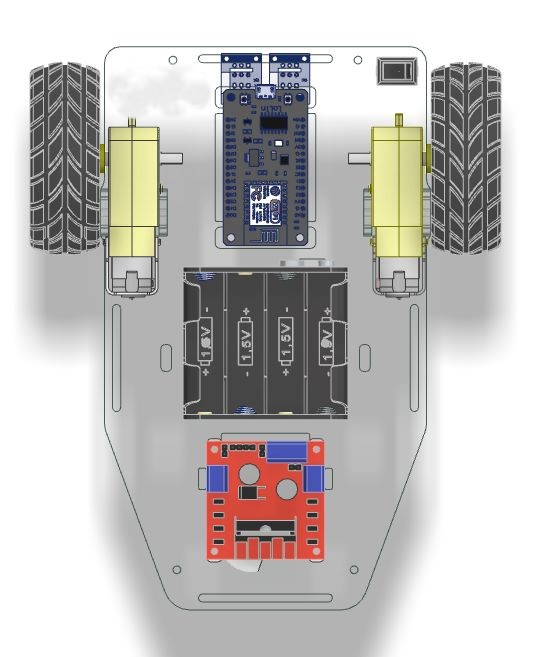
\includegraphics[width=0.3\linewidth]{../Gambar/rancnaganrobot.jpg}
  \caption{Rancangan desain robot}
  \label{fig:rancanganrobot}
\end{figure}
